% !TEX root = ../../../main.tex
% 来源：中学数学实验教材·第三册（高中数学）
% 章节：指数概念普遍化与对数 / 对数和常用对数
% 原始文件：1.tex，行 2705-2713
% 类型：tikz
% ---
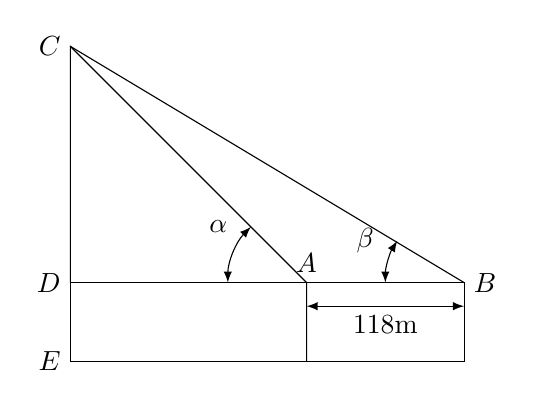
\begin{tikzpicture}[scale=1, >=latex]
\draw (0,0)node[left]{$E$} rectangle (5,1);
\draw (0,1)node[left]{$D$}--(0,4)node[left]{$C$}--(5,1)node[right]{$B$};
\draw (0,4)--(3,1)node[above]{$A$}--(3,0);

\draw[<->] (2,1) arc (180:90+45:1)node[left=5pt]{$\alpha$};
\draw[<->] (4,1) arc (180:180-32:1)node[left=5pt]{$\beta$};
\draw[<->] (5,.7) --node[below]{118m}(3,.7);
\end{tikzpicture}
